\section{REQUIREMENTS, DESIGN AND IMPLEMENTATION}
\subsection{Actors}
\begin{itemize}
	\item \textbf{Fleet manager}, who performs the following activities:
	\begin{itemize}
		\item Login.
		\item Get bus location.
		\item Add/Remove/Modify bus.
		\item Assign drivers to buses.
		\item Add/Remove route.
		\item Add/Remove/Modify driver.
		\item View the user requests on a map.
		\item View previous user requests.
		\item View routes utilization.
	\end{itemize}
	\item \textbf{Bus driver}, who performs the following activities:
	\begin{itemize}
		\item Login.
		\item View schedule with user requests.
	\end{itemize}
	\item \textbf{Passenger}, who generates the user requests for a bus, specifying at which stop he/she wants to get on and off the bus.
\end{itemize}

\subsection{Functional Requirements}
\subsubsection{Use case}
\begin{figure}[H]
	\centering
	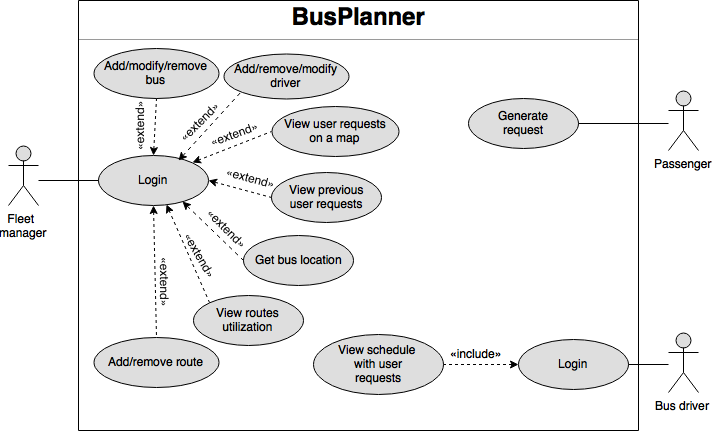
\includegraphics[width=14cm]{UseCase}
\end{figure}

\subsubsection{User stories}
\begin{table}[H]
	\centering
	\begin{tabular}{| m{2.2cm} | m{6cm} | m{3.8cm} |}
		\hline
		\textbf{ID} & \textbf{User story} & \textbf{Sprint} \\
		\hline
		UserStory1 & As fleet manager I want to be able to log into (or logout) the system with my account at any time. & Done in Sprint 1.\\
		\hline
		UserStory2 & As fleet manager I want to be able to add, modify or remove a bus. & Done in Sprint 1.\\
		\hline
		UserStory3 & As fleet manager I want to be able to add, modify or remove a driver. & Done in Sprint 2.\\
		\hline
		UserStory4 & As fleet manager I want to be able to view user requests on a map. & Done in Sprint 3.\\
		\hline
		UserStory5 & As fleet manager I want to be able to view previous user requests. & Done in Sprint 3.\\
		\hline
		UserStory6 & As fleet manager I want to be able to get the position of all the buses. & Done in Sprint 2.\\
		\hline
		UserStory7 & As fleet manager I want to be able to get the utilization of all the routes. & Done in Sprint 3.\\
		\hline
		UserStory8 & As fleet manager I want to be able to add or remove a route. & Done in Sprint 2.\\
		\hline
		UserStory9 & As a bus driver I want to be able to log into (or logout) the system with my account at any time. & Done in Sprint 1.\\
		\hline
		UserStory10 & As a bus driver I want to be able to see the schedule of the route I have to cover, with the user requests I need to satisfy. & Done in Sprint 2.\\
		\hline
	\end{tabular}
\end{table}
\newpage
\subsection{Nonfunctional Requirements}
This section presents the nonfunctional requirements of our BusPlanner project, which describe the behavior of the system. We decided to divide them into 7 main categories.
\subsubsection{Usability}
\begin{itemize}
	\item The application must be mobile responsive.
	\item The seat reservation should be done in the minimum number of steps possible.
	\item No fancy GUI.
	\item Correct and up to date information.
	\item Presenting data in a visible and understandable way.	
\end{itemize}
\subsubsection{External Libraries}
\begin{itemize}
	\item Our application makes usage of external libraries such as Bootstrap.
\end{itemize}
\subsubsection{Compatibility issue}
\begin{itemize}
	\item The application is suggested to work only with the deployed version of the used libraries. Updated versions might bring incompatibilities. 
	\item The maps being used should offer the possibility to work with PHP and SQL.
\end{itemize}
\subsubsection{Security}
\begin{itemize}
	\item Only users of the application are allowed to use the project. 
	\item The application needs to protect C.I.A elements (Confidentiality, Integrity and Availability) of user and nobody can see and change information of others.
\end{itemize}
\newpage
\subsubsection{Availability}
Considering that the application:
\begin{itemize}
	\item Can pave the way for users to take a bus as soon as possible with the aim of saving their time.
	\item Can make it easier for users to take a bus from everywhere in bus timetable.
	\item Can have friendly interface for users.
	\item Performance should provide the user a fast experience using the application.
	\item Has to handle user\textquotesingle s request all the time using any device with an Internet connection and an installed web browser.
\end{itemize}

\subsubsection{Uptime and data redundancy}
The BusPlanner application should guarantee high availability and data redundancy. Still, since the application will be created in the context of the DSD course, our team will not build nor require any dedicated infrastructure for it and so estimating and proving exact value for data redundancy and uptime is not possible; however, in the case there\textquotesingle s the chance to build and test a dedicated infrastructure, an uptime of at least 99.99\% is desirable along with at least one database replication.

\subsubsection{Performances}
The application has to be able to manage a high volume of requests. Since this application will be created in the context of the DSD course, our team will not build nor require any dedicated infrastructure for it. Furthermore, it is impossible to estimate and prove the exact value for performances. However, it should be easy to update it and improve it if needed. 

\subsection{High-Level Architecture}
\begin{figure}[H]
	\centering
	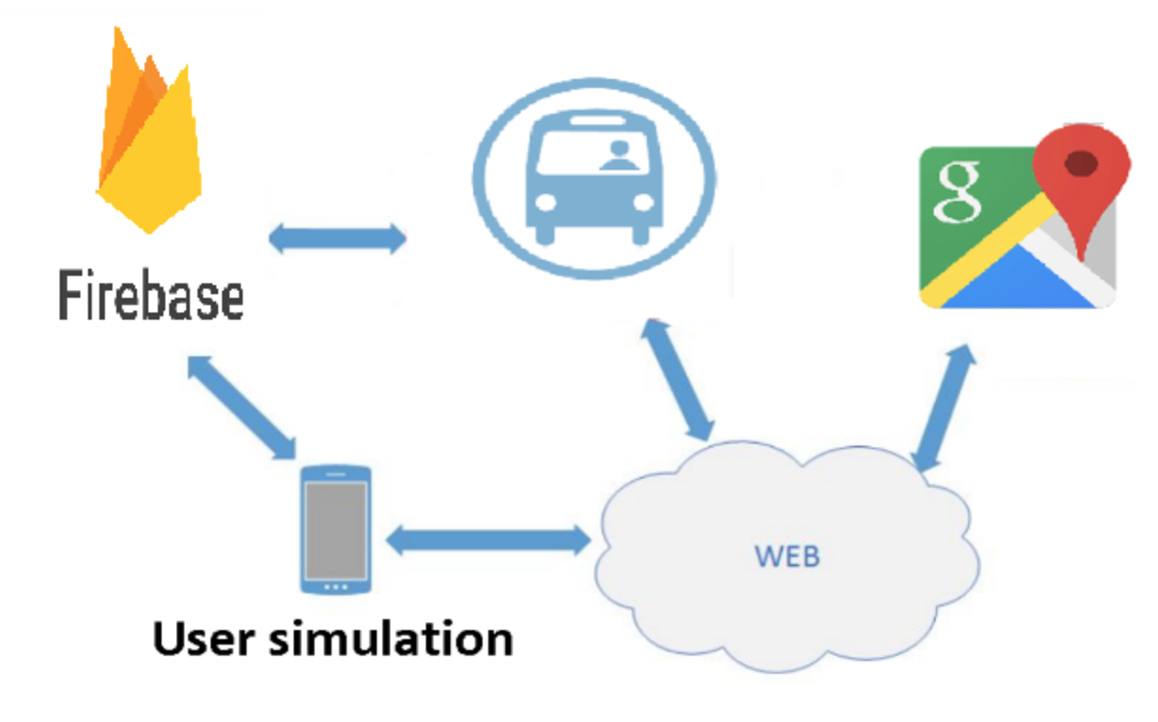
\includegraphics[width=12cm]{SystemArchitecture}
\end{figure}

\subsection{Technologies used}
\begin{figure}[H]
	\centering
	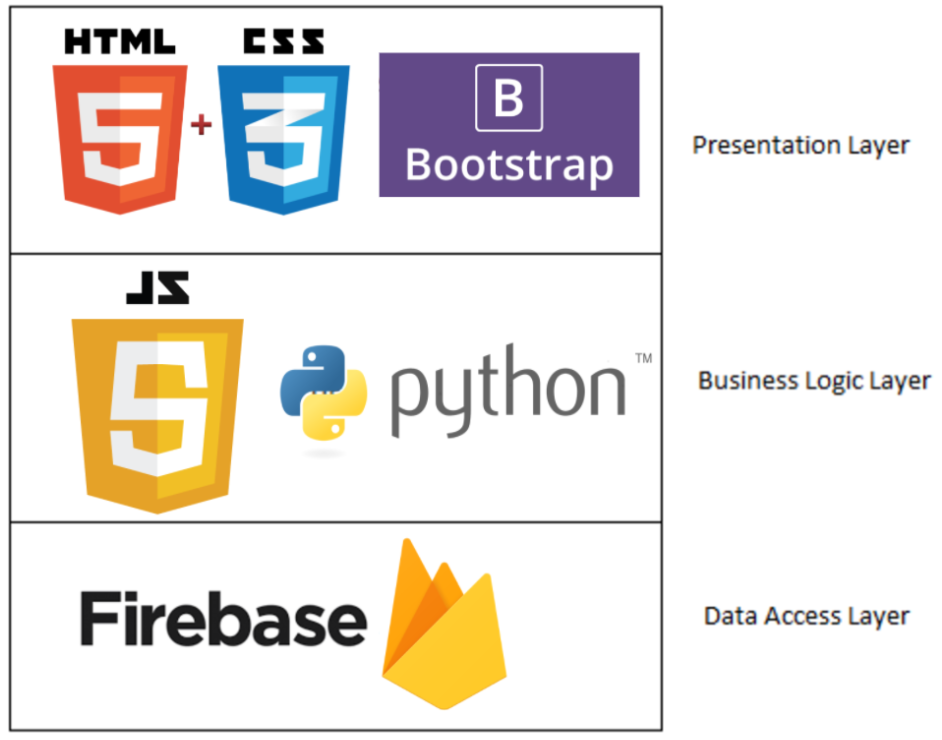
\includegraphics[width=12cm]{TechnologiesUsed}
\end{figure}

\subsection{Algorithm}
The algorithm is divided into static algorithm and dynamic algorithm.

\subsubsection{Static Algorithm}
It has been implemented by Andrea Colombo and Huy Hoang Nguyen.

The programming language used for its implementation was Python, with the addition of some libraries. It covers the simulation of user requests with the generation of timetables based on those requests. So, for the generation of timetables, the algorithm takes in input the user requests and produces the corresponding timetables.

The user requests are simulated through a Poisson distribution, based on the current time and a delta time that will then be added to cover all times of the day. The number of user requests for each time slot of the day depends on the lambda parameter of the Poisson distribution.

The intermediate passage is characterized by the grouping of user requests per route, that will later be sorted by time. Finally, the algorithm has to calculate all timetables elements (i.e. number of onboarding/deboarding passengers, departure and arrival time etc.).

\begin{figure}[H]
	\centering
	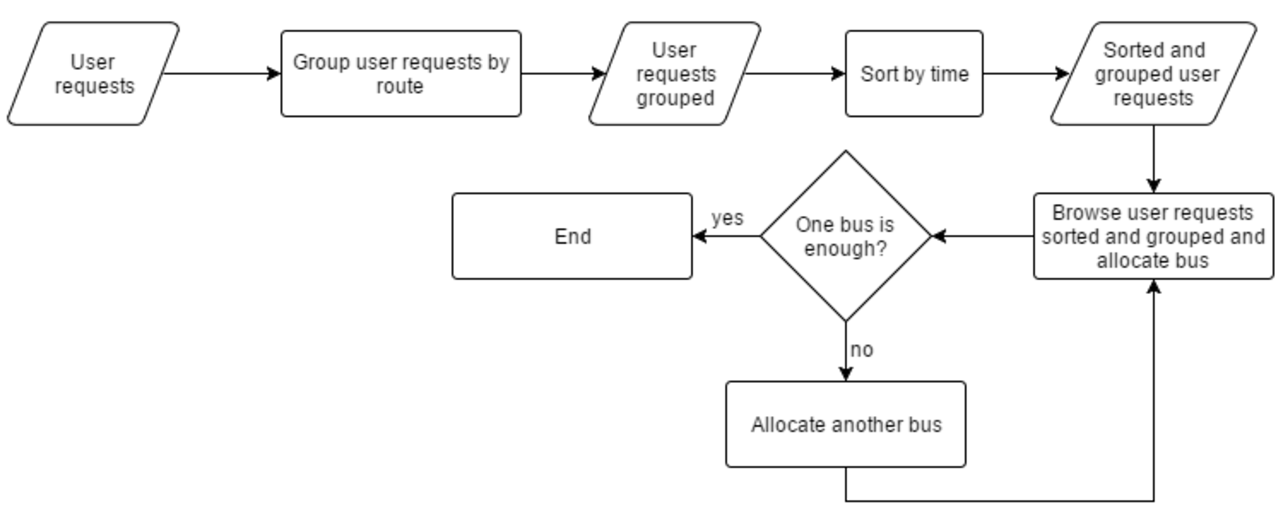
\includegraphics[width=14cm]{Flowchart}
	\caption{Static algorithm flowchart}
\end{figure}
\newpage
\subsubsection{Dynamic Algorithm}
It has been implemented by Albi Dode and Sharvathul Hasan Ameerjan.

The programming language used for its implementation was Python, with the addition of some libraries and Linear Programming.

The initial idea was that we should have had one bus per route at a certain point of time, and each bus had to start and end at the bus depot.

The algorithm takes in input the number of onboarding and deboarding passengers and the starting and ending working hour of bus drivers, and produces as output the number of trips that a bus driver can do, the connection between time and trip and the route-bus assignment. 

Since we had to implement a lot of requirements, which caused a lot of if \& else statements, Linear Programming was used in order to fulfill certain criteria (named as rules in the code) and minimize some objective function.

The goal is to satisfy as many trips as possible in one duty.